\chapter{Desenvolvimento} % TODO: Melhorar isso no futuro e resumir a primeira parte

Esta seção apresenta as duas etapas do desenvolvimento do trabalho. Para cada etapa, será apresentado o processo de
treinamento e de execução de testes, incluindo também a análise dos resultados. Essa divisão permite uma análise mais
aprofundada dos experimentos com diferentes conjuntos de dados.

\section{Tecnologias Utilizadas}

Para ambas as etapas, as mesmas tecnologias foram utilizadas. O processamento de dados e \textit{fine-tuning} foram
feitos com \textit{scripts} em Python e \textit{Jupyter notebooks}. Já as dependências do projeto foram gerenciadas com
o gerenciador Poetry e o \textit{framework} de \textit{fine-tuning} utilizado foi o Unsloth. Por fim, os treinamentos
foram realizados com uma placa NVIDIA H100 de 80 GB que faz parte de uma plataforma NVIDIA DGX H100.

\section{Etapa Inicial de Desenvolvimento}

Nesta seção, a etapa inicial de \textit{fine-tuning} do \ac{LLaMA}-3.2 é apresentada, sendo que ela tem um caráter
exploratório e visa o desenvolvimento do código base para os próximos experimentos e a análise da capacidade
de classificação do modelo quando treinado de diferentes formas. Nesta etapa o modelo é treinado para classificar
imagens de lesão de pele advindas de dermatoscopia.

\subsection{Conjunto de Dados}

Para os experimentos iniciais, utilizou-se o conjunto de dados \ac{HAM10000} de \textcite{tschandl2018ham10000}, que
possui 13354 imagens de dermatoscopia com informações como a doença causadora da lesão de pele, a idade do paciente,
sexo e localização da lesão.

O conjunto de dados é separado nas seções de treinamento, teste e validação, que possuem 9577, 1285 e 2492 imagens,
respectivamente. A \autoref{tab:ham10000_proportion} apresenta as proporções entre as categorias de lesões de pele. Os
dados foram obtidos a partir da plataforma Hugging Face com uma versão do \ac{HAM10000} fornecida por
\textcite{skin_cancer_dataset}. A proporção das lesões é conservada entre as seções do conjunto de dados.

\begin{table}[ht]
    \caption{\small Proporção entre as diferentes categorias de lesões de pele no \ac{HAM10000}.}
    \centering
    \begin{tabular}{l|c}
        \hline
        Lesão de pele                        & Proporção (\%) \\ \hline
        Nevo melanocítico                    & 66,88          \\
        Melanoma                             & 11,23          \\
        Lesões similares à queratose benigna & 10,94          \\
        \ac{CBC}                             & 5,08           \\
        Queratose actínica                   & 3,29           \\
        Lesões vasculares                    & 1,42           \\
        Dermatofibroma                       & 1,15           \\ \hline
    \end{tabular}
    \label{tab:ham10000_proportion}
    \fonte{\textcite{tschandl2018ham10000}}
\end{table}

\subsection{Experimentos com \textit{Fine-tuning}}

Os experimentos utilizaram a variante \ac{LLaMA}-3.2-11B-Vision-Instruct, que possui 11 bilhões de parâmetros. Os
métodos de \textit{fine-tuning} utilizados foram o \ac{LoRA} e o \ac{QLoRA}.

\subsubsection{Dados de Treinamento}

Para treinar o modelo, foram gerados diálogos constituídos de um pedido para a classificação da lesão com base em uma
imagem e de uma resposta com a classe da lesão. Os pares de imagens e lesões de pele foram selecionados a partir de
amostras do conjunto de dados de treinamento. A amostragem foi feita com base nas classes das lesões de pele, assim,
cada amostra possui uma representação proporcional de lesões em relação ao conjunto de dados completo.

Durante a execução desta etapa, o modelo utilizado ainda não suportava a utilização de textos em português para tarefas
multimodais, sendo assim, os diálogos estão em inglês. O diálogo pode ser conferido abaixo:

\begin{dialogue}
    \speak{Usuário} \textit{Classify the skin lesion in the image. \textbf{<imagem>}} \\
    \speak{Modelo} \textit{The skin lesion in the image is \textbf{<lesão de pele>}.}
\end{dialogue}

\subsubsection{\textit{Fine-tuning} com 450, 900 e 1800 Amostras}

A primeira etapa nos experimentos foi a realização o \textit{fine-tuning} com \ac{QLoRA} com 450 amostras de
treinamento e 50 de validação. Os hiperparâmetros\footnote{parâmetros de treinamento} utilizados no treinamento estão
na \autoref{tab:qlora_500_config}, alguns deles foram omitidos por serem menos relevantes nessa etapa. O \ac{rsLoRA} de
\textcite{kalajdzievski2023rank} foi utilizado para melhorar o desempenho, utilizando um fator de escala
\begin{math}\frac{\alpha_{LoRA}}{\sqrt{r}}\end{math} em vez do \begin{math}\frac{\alpha_{LoRA}}{r}\end{math} do
\ac{LoRA} original. Por fim, também foi utilizado o otimizador \ac{Adam} na sua versão paginada de 32 bits. A
\autoref{tab:qlora_500_training} apresenta dados sobre o treinamento e a \autoref{fig:loss_qlora_500} apresenta o
\textit{loss} de treinamento e validação ao longo dos passos.

\begin{table}[ht]
    \caption{\small Hiperparâmetros para o \ac{QLoRA} com 450, 900 e 1800 amostras. A primeira seção se refere às
    configurações
    específicas de \ac{PEFT}, enquanto a
    segunda se refere ao treinamento em geral.}
    \centering
    \begin{tabular}{l|c}
        \hline
        Hiperparâmetro                             & Valor                                  \\ \hline
        Camadas e módulos treinados                & Visão, linguagem, atenção e \ac{MLP}   \\
        Rank                                       & 32                                     \\
        Alfa (\begin{math}\alpha_{LoRA}\end{math}) & 32                                     \\
        Dropout                                    & 0,1                                    \\
        \ac{rsLoRA}                                & Sim                                    \\ \hline
        Taxa de aprendizado                        & \begin{math}2 \times 10^{-4}\end{math} \\
        Razão de aquecimento                       & 0,03                                   \\
        Tipo de escalonador da taxa de aprendizado & Cosseno com reinícios                  \\
        Decaimento de peso                         & 0,01                                   \\
        Épocas                                     & 5                                      \\
        Passos a cada validação                    & 50                                     \\
        Otimizador                                 & \ac{Adam} paginado de 32 bits          \\
        Tipo numérico                              & \ac{BF16}                              \\ \hline
    \end{tabular}
    \label{tab:qlora_500_config}
    \fonte{Autoria própria}
\end{table}

\begin{table}[ht]
    \caption{\small Dados sobre o treinamento com \ac{QLoRA} com 450 amostras.}
    \centering
    \begin{tabular}{l|c}
        \hline
                                    & Valor     \\ \hline
        Parâmetros treináveis       & 134348800 \\
        Tempo de treinamento (min)  & 16,17     \\
        Passos                      & 110       \\
        Memória máxima alocada (GB) & 18.69     \\ \hline
    \end{tabular}
    \label{tab:qlora_500_training}
    \fonte{Autoria própria}
\end{table}

\begin{figure}[ht]
    \centering
    \caption{\small \textit{Loss} de treinamento e validação para o \ac{QLoRA} com 450 amostras.}
    
\includegraphics[width=0.8\columnwidth,keepaspectratio]{images/loss_qlora_500.png}
    \label{fig:loss_qlora_500}
    \fonte{Autoria própria.}
\end{figure}

Em seguida, foi realizado o \textit{fine-tuning} com \ac{LoRA}, ou seja, sem quantização, com 450 amostras. Os
hiperparâmetros utilizados são similares, porém, o \textit{rank} foi reduzido para 16, assim como o
\begin{math}\alpha_{LoRA}\end{math}. O
\ac{rsLoRA} não foi utilizado e a taxa de aprendizado foi reduzida a
\begin{math}1 \times 10^{-4}\end{math}. Por fim o otimizador \ac{AdamW} foi utilizado. A
\autoref{tab:lora_500_training} apresenta os dados
de treinamento e a
\autoref{fig:loss_lora_500} apresenta o \textit{loss}. O treinamento foi aplicado somente sobre 64174400 parâmetros,
uma quantidade menor
do que a usada no
\ac{QLoRA} por conta do \textit{rank} reduzido.

\begin{table}[ht]
    \caption{\small Dados sobre o treinamento com \ac{LoRA} com 450 amostras.}
    \centering
    \begin{tabular}{l|c}
        \hline
                                    & Valor    \\ \hline
        Parâmetros treináveis       & 64174400 \\
        Tempo de treinamento (min)  & 26,42    \\
        Passos                      & 140      \\
        Memória máxima alocada (GB) & 40,35    \\ \hline
    \end{tabular}
    \label{tab:lora_500_training}
    \fonte{Autoria própria}
\end{table}

\clearpage

\begin{figure}[ht]
    \centering
    \caption{\small \textit{Loss} de treinamento e validação para o \ac{LoRA} com 450 amostras.}
    
\includegraphics[width=0.725\columnwidth,keepaspectratio]{images/loss_lora_500.png}
    \label{fig:loss_lora_500}
    \fonte{Autoria própria.}
\end{figure}

O \textit{fine-tuning} com 900 amostras foi feito sem a alteração nos hiperparâmetros do \ac{QLoRA} e \ac{LoRA}. As
informações sobre o treinamento podem ser conferidas na \autoref{tab:qlora_1000_training} e
\autoref{tab:lora_1000_training}, enquanto o \textit{loss} pode ser conferido na \autoref{fig:loss_qlora_1000} e
\autoref{fig:loss_lora_1000}.

\begin{table}[ht]
    \caption{\small Dados sobre o treinamento com \ac{QLoRA} com 900 amostras.}
    \centering
    \begin{tabular}{l|c}
        \hline
                                    & Valor     \\ \hline
        Parâmetros treináveis       & 134348800 \\
        Tempo de treinamento (min)  & 32,08     \\
        Passos                      & 225       \\
        Memória máxima alocada (GB) & 18,695    \\ \hline
    \end{tabular}
    \label{tab:qlora_1000_training}
    \fonte{Autoria própria}
\end{table}

\begin{table}[ht]
    \caption{\small Dados sobre o treinamento com \ac{LoRA} com 900 amostras.}
    \centering
    \begin{tabular}{l|c}
        \hline
                                    & Valor    \\ \hline
        Parâmetros treináveis       & 67174400 \\
        Tempo de treinamento (min)  & 41,76    \\
        Passos                      & 280      \\
        Memória máxima alocada (GB) & 31,965   \\ \hline
    \end{tabular}
    \label{tab:lora_1000_training}
    \fonte{Autoria própria}
\end{table}

\clearpage

\begin{figure}[ht]
    \centering
    \caption{\small \textit{Loss} de treinamento e validação para o \ac{QLoRA} com 900 amostras.}
    
\includegraphics[width=0.725\columnwidth,keepaspectratio]{images/loss_qlora_1000.png}
    \label{fig:loss_qlora_1000}
    \fonte{Autoria própria.}
\end{figure}

\begin{figure}[ht]
    \centering
    \caption{\small \textit{Loss} de treinamento e validação para o \ac{LoRA} com 900 amostras.}
    
\includegraphics[width=0.725\columnwidth,keepaspectratio]{images/loss_lora_1000.png}
    \label{fig:loss_lora_1000}
    \fonte{Autoria própria.}
\end{figure}

Por último, foi feito um \textit{fine-tuning} com \ac{QLoRA} com 1800 amostras com os mesmos hiperparâmetros utilizados
anteriormente. As informações sobre o treinamento podem ser vistas na \autoref{tab:qlora_2000_training} e na
\autoref{fig:loss_qlora_2000}.

\clearpage

\begin{table}[ht]
    \caption{\small Dados sobre o treinamento com \ac{QLoRA} com 1800 amostras.}
    \centering
    \begin{tabular}{l|c}
        \hline
                                    & Valor     \\ \hline
        Parâmetros treináveis       & 134348800 \\
        Tempo de treinamento (min)  & 90,77     \\
        Passos                      & 450       \\
        Memória máxima alocada (GB) & 18,744    \\ \hline
    \end{tabular}
    \label{tab:qlora_2000_training}
    \fonte{Autoria própria}
\end{table}

\begin{figure}[ht]
    \centering
    \caption{\small \textit{Loss} de treinamento e validação para o \ac{QLoRA} com 1800 amostras.}
    
\includegraphics[width=0.725\columnwidth,keepaspectratio]{images/loss_qlora_2000.png}
    \label{fig:loss_qlora_2000}
    \fonte{Autoria própria.}
\end{figure}

\subsubsection{\textit{Fine-tuning} com 5000 e 9500 Amostras}

Para avaliar o impacto de diferentes hiperparâmetros, foram feitos \textit{fine-tunings} modificados com 5000 e 9500
amostras. As configurações na \autoref{tab:qlora_5000_config} se referem tanto ao \ac{QLoRA} quanto ao \ac{LoRA}. Foi
utilizado somente o \ac{QLoRA} no treinamento com 9500 amostras. Os dados dos treinamentos podem ser conferidos na
\autoref{tab:qlora_5000_training}, \autoref{tab:lora_5000_training} e \autoref{tab:qlora_9500_training}, enquanto o
\textit{loss} pode ser conferido na \autoref{fig:loss_qlora_5000}, \autoref{fig:loss_lora_5000} e
\autoref{fig:loss_qlora_9500}.

\clearpage

\begin{table}[ht]
    \caption{\small Hiperparâmetros para o \textit{fine-tuning} com 5000 e 9500 amostras. A primeira seção se refere às
    configurações
    específicas de \ac{PEFT}, enquanto
    a segunda se refere ao treinamento em geral.}
    \centering
    \begin{tabular}{l|c}
        \hline
        Hiperparâmetro                             & Valor                                  \\ \hline
        Camadas e módulos treinados                & Visão, linguagem, atenção e \ac{MLP}   \\
        Rank                                       & 64                                     \\
        Alfa (\begin{math}\alpha_{LoRA}\end{math}) & 64                                     \\
        Dropout                                    & 0,05                                   \\
        \ac{rsLoRA}                                & Sim                                    \\ \hline
        Taxa de aprendizado                        & \begin{math}1 \times 10^{-4}\end{math} \\
        Razão de aquecimento                       & 0                                      \\
        Tipo de escalonador da taxa de aprendizado & Constante                              \\
        Decaimento de peso                         & 0,01                                   \\
        Épocas                                     & 3                                      \\
        Passos a cada validação                    & A cada 5\% dos passos                  \\
        Otimizador                                 & \ac{Adam} paginado de 32 bits          \\
        Tipo numérico                              & \ac{BF16}                              \\ \hline
    \end{tabular}
    \label{tab:qlora_5000_config}
    \fonte{Autoria própria}
\end{table}

\begin{table}[ht]
    \caption{\small Dados sobre o treinamento com \ac{QLoRA} com 5000 amostras.}
    \centering
    \begin{tabular}{l|c}
        \hline
                                    & Valor     \\ \hline
        Parâmetros treináveis       & 268697600 \\
        Tempo de treinamento (min)  & 96,63     \\
        Passos                      & 1875      \\
        Memória máxima alocada (GB) & 18,967    \\ \hline
    \end{tabular}
    \label{tab:qlora_5000_training}
    \fonte{Autoria própria}
\end{table}

\begin{table}[ht]
    \caption{\small Dados sobre o treinamento com \ac{LoRA} com 5000 amostras.}
    \centering
    \begin{tabular}{l|c}
        \hline
                                    & Valor     \\ \hline
        Parâmetros treináveis       & 268697600 \\
        Tempo de treinamento (min)  & 100,33    \\
        Passos                      & 1875      \\
        Memória máxima alocada (GB) & 31,48     \\ \hline
    \end{tabular}
    \label{tab:lora_5000_training}
    \fonte{Autoria própria}
\end{table}

\clearpage

\begin{table}[ht]
    \caption{\small Dados sobre o treinamento com \ac{QLoRA} com 9500 amostras.}
    \centering
    \begin{tabular}{l|c}
        \hline
                                    & Valor     \\ \hline
        Parâmetros treináveis       & 268697600 \\
        Tempo de treinamento (min)  & 177,44    \\
        Passos                      & 3564      \\
        Memória máxima alocada (GB) & 18,971    \\ \hline
    \end{tabular}
    \label{tab:qlora_9500_training}
    \fonte{Autoria própria}
\end{table}

\begin{figure}[ht]
    \centering
    \caption{\small \textit{Loss} de treinamento e validação para o \ac{QLoRA} com 5000 amostras.}
    
\includegraphics[width=0.725\columnwidth,keepaspectratio]{images/loss_qlora_5000.png}
    \label{fig:loss_qlora_5000}
    \fonte{Autoria própria.}
\end{figure}

\clearpage

\begin{figure}[ht]
    \centering
    \caption{\small \textit{Loss} de treinamento e validação para o \ac{LoRA} com 5000 amostras.}
    
\includegraphics[width=0.725\columnwidth,keepaspectratio]{images/loss_lora_5000.png}
    \label{fig:loss_lora_5000}
    \fonte{Autoria própria.}
\end{figure}

\begin{figure}[ht]
    \centering
    \caption{\small \textit{Loss} de treinamento e validação para o \ac{QLoRA} com 9500 amostras.}
    
\includegraphics[width=0.725\columnwidth,keepaspectratio]{images/loss_qlora_9500.png}
    \label{fig:loss_qlora_9500}
    \fonte{Autoria própria.}
\end{figure}

\subsubsection{Análise dos Treinamentos}

A vantagem no baixo gasto de memória do \ac{QLoRA} se torna evidente com os treinamentos, usando em média 1,8 vezes
menos memória que o \ac{LoRA}. Observa-se também que as configurações de \textit{fine-tuning} usadas no treinamento com
5000 e 9500 amostras levaram a uma maior instabilidade no \textit{loss} do longo dos passos.

\subsection{Testes}

Os testes se consistiram em uma série de perguntas aos modelos, em que foram usadas duas modalidades de pergunta, uma
livre e outra objetiva. Na pergunta livre o \textit{prompt} é definido como:

\begin{dialogue}
    \speak{Usuário} \textit{Classify the skin lesion in the image. \textbf{<imagem>}}
\end{dialogue}

Já na pergunta objetiva, é esperado que o modelo informe apenas o nome da doença com base nas opções possíveis do
conjunto de dados, sendo que o \textit{prompt} usado é:

\begin{dialogue}
    \speak{Usuário} \textit{Classify the skin lesion in the image. Say only the name of the disease and nothing else.
    The diseases to
    be classified are: melanocytic Nevi,
    melanoma, benign keratosis-like lesions, basal cell carcinoma, actinic keratoses, vascular lesions and
    dermatofibroma.\textbf{<imagem>}}
\end{dialogue}

Foram feitas 100 perguntas livres e 1000 perguntas objetivass para cada modelo treinado e para o
\ac{LLaMA}-3.2-11B-Vision-Instruct na versão normal e na quantizada. As imagens utilizadas vieram da seção de teste do
conjunto de dados. A \textit{temperatura}, uma variável que define a previsibilidade do modelo, foi definida como 0,1
para que as respostas fossem mais precisas. Além disso, o número máximo de \textit{tokens} foi definido como 128.

\subsection{Análise dos Resultados da Iniciais}

Os testes com perguntas livres foram avaliados manualmente para observar o formato de resposta dos modelos, enquanto os
testes com perguntas objetivas foram processados para a extração das lesões previstas para as imagens. Com esses dados,
foram geradas matrizes de confusão com os cálculos da acurácia de cada modelo.

\subsubsection{Análise do LLaMA-3.2-Vision-Instruct}

Tanto o modelo na versão normal quanto o modelo quantizado apresentaram respostas bem variadas para cada pergunta
livre. Em geral, as respostas apresentam uma estrutura de passos que se baseia em metodologias de classificação de
lesões de pele. O diálogo abaixo apresenta uma classificação correta para a imagem de um melanoma:

\begin{dialogue}
    \speak{Usuário} \textit{Classify the skin lesion in the image. \textbf{<imagem de um melanoma>}} \\
    \speak{Modelo} \textit{\textbf{Step 1: Identify the lesion.} \\
    The image shows a skin lesion with an irregular border and a dark brown color. \\
    \textbf{Step 2: Determine the characteristics of the lesion.} \\
    The lesion has an irregular border, which is a characteristic of melanoma. The dark brown color is also consistent
    with
    melanoma. \\
    \textbf{Step 3: Consider the possible diagnoses.} \\
    Based on the characteristics of the lesion, it is likely that the diagnosis is melanoma. \\
    \textbf{Step 4: Provide the final answer.} \\
    \textbf{Answer:} Melanoma}
\end{dialogue}

Muitas respostas apresentaram uma classificação incorreta, embora tenham sido descritivas sobre a lesão. No exemplo
abaixo, o modelo classificou um nevo melanocítico como um melanoma:

\begin{dialogue}
    \speak{Usuário} \textit{Classify the skin lesion in the image. \textbf{<imagem de um nevo melanocítico>}} \\
    \speak{Modelo} \textit{\textbf{Step 1: Identify the lesion} \\
    The image shows a brown, irregularly shaped lesion with a darker brown border. \\
    \textbf{Step 2: Determine the characteristics of the lesion} \\
    The lesion is asymmetrical, has an irregular border, and has multiple colors. \\
    \textbf{Step 3: Classify the lesion} \\
    Based on the characteristics of the lesion, it is classified as a melanoma. \\
    \textbf{Answer:} Melanoma}
\end{dialogue}

Algumas respostas não apresentaram uma classificação precisa, sendo que o modelo informou apenas que a imagem se
tratava de uma lesão de pele. Um exemplo assim pode ser visto no diálogo abaixo:

\begin{dialogue}
    \speak{Usuário} \textit{Classify the skin lesion in the image. \textbf{<imagem de um nevo melanocítico>}} \\
    \speak{Modelo} \textit{The skin lesion in the image appears to be a dermatological condition, likely a typeof skin
    cancer or a
    benign growth. However, without
    further information or a medical diagnosis, it is difficult to provide a definitive classification.}
\end{dialogue}

Já nas respostas às perguntas objetivas, o modelo quantizado teve um desempenho levemente pior em relação ao não
quantizado. Porém, ambos tiveram um desempenho pouco satisfatório, a versão quantizada atingiu apenas 11,8\% de
acurácia e a não quantizada atingiu 14\%.

A \autoref{fig:confusion_matrix_llama_quantized} e a \autoref{fig:confusion_matrix_llama} apresentam as matrizes de
confusão normalizadas pelos valores verdadeiros para o modelo quantizado e o não quantizado, respectivamente. Nota-se
que eles classificaram as lesões como melanoma em uma escala desproporcional, o \ac{LLaMA} quantizado classificou
97,6\% das lesões como melanoma, enquanto o não quantizado classificou 88,3\%. Também pode-se notar uma tendência da
classificação de lesões vasculares como dermatofibroma por parte do modelo não quantizado.

Foram registradas 3 respostas incertas para o modelo quantizado e apenas uma para o não quantizado.

\begin{figure}[ht]
    \centering
    \caption{\small Matriz de confusão para o \ac{LLaMA}-11B-Vision-Instruct quantizado.}

    
\includegraphics[width=1\columnwidth,keepaspectratio]{images/confusion_matrix_llama_3.2_11b_vision_instruct_quantized.png}
    \label{fig:confusion_matrix_llama_quantized}
    \fonte{Autoria própria.}
\end{figure}

\clearpage

\begin{figure}[ht]
    \centering
    \caption{\small Matriz de confusão para o \ac{LLaMA}-11B-Vision-Instruct.}
    
\includegraphics[width=1\columnwidth,keepaspectratio]{images/confusion_matrix_llama_3.2_11b_vision_instruct.png}
    \label{fig:confusion_matrix_llama}
    \fonte{Autoria própria.}
\end{figure}

\subsubsection{Análise dos Modelos após o \textit{fine-tuning}}

Para as perguntas livres, todos os modelos treinados responderam no formato especificado no treinamento. O primeiro
diálogo abaixo apresenta uma classificação correta e o segundo apresenta uma incorreta, ambas as respostas foram dadas
pelo modelo treinado com \ac{QLoRA} com 450 amostras:

\begin{dialogue}
    \speak{Usuário} \textit{Classify the skin lesion in the image. \textbf{<imagem de um nevo melanocítico>}} \\
    \speak{Modelo} \textit{The skin lesion in the image is melanocytic Nevi.}
\end{dialogue}

\begin{dialogue}
    \speak{Usuário} \textit{Classify the skin lesion in the image. \textbf{<imagem de um nevo melanoma>}} \\
    \speak{Modelo} \textit{The skin lesion in the image is benign keratosis-like lesions.}
\end{dialogue}

Os modelos trainados com \ac{QLoRA} com 450, 5000 e 9500 amostras, e com \ac{LoRA} com 5000 amostras apresentaram um
problema em que as respostas não obedecem ao formato especificado na pergunta objetiva, respondendo com o texto
completo.

A acurácia nas respostas às perguntas objetivas aumentou consideravelmente com o \textit{fine-tuning} com \ac{QLoRA},
chegando a atingir 65,5\%. Porém, o modelo gerado com esse treinamento tende a classificar a maioria das lesões como
nevo melanocítico, o que indica que a acurácia maior pode ser simplesmente devido a uma quantidade maior de nevos
melanocíticos nos dados de teste. Para o modelo treinado com \ac{LoRA}, o desempenho foi menor, atingindo apenas 49,5\%
de acurácia.

Em geral, como pode ser visto na \autoref{fig:confusion_matrix_qlora_450} e \autoref{fig:confusion_matrix_lora_450}, as
duas versões ficaram insatisfatórias, o que se deve a um treinamento com um conjunto pequeno de dados e hiperparâmetros
não ideais.

\begin{figure}[ht]
    \centering
    \caption{\small Matriz de confusão para o \ac{LLaMA} treinado com \ac{QLoRA} e 450 amostras.}
    
\includegraphics[width=1\columnwidth,keepaspectratio]{images/confusion_matrix_qlora_450.png}
    \label{fig:confusion_matrix_qlora_450}
    \fonte{Autoria própria.}
\end{figure}

\clearpage

\begin{figure}[ht]
    \centering
    \caption{\small Matriz de confusão para o \ac{LLaMA} treinado com \ac{LoRA} e 450 amostras.}
    
\includegraphics[width=1\columnwidth,keepaspectratio]{images/confusion_matrix_lora_450.png}
    \label{fig:confusion_matrix_lora_450}
    \fonte{Autoria própria.}
\end{figure}

A acurácia decaiu levemente no \textit{fine-tuning} com 900 amostas, conforme apresentado na
\autoref{fig:confusion_matrix_qlora_900} e \autoref{fig:confusion_matrix_lora_900}, ficando em 65.2\% para o \ac{LLaMA}
treinado com \ac{QLoRA} e 42\% para o treinado com \ac{LoRA}. Porém, o modelo treinado com \ac{QLoRA} apresenta um
padrão melhor de classificação, reconhecendo melhor as lesões de nevos melanocíticos e de queratoses actínicas.

\clearpage

\begin{figure}[ht]
    \centering
    \caption{\small Matriz de confusão para o \ac{LLaMA} treinado com \ac{QLoRA} e 900 amostras.}
    
\includegraphics[width=1\columnwidth,keepaspectratio]{images/confusion_matrix_qlora_900.png}
    \label{fig:confusion_matrix_qlora_900}
    \fonte{Autoria própria.}
\end{figure}

\clearpage

\begin{figure}[ht]
    \centering
    \caption{\small Matriz de confusão para o \ac{LLaMA} treinado com \ac{LoRA} e 900 amostras.}
    
\includegraphics[width=1\columnwidth,keepaspectratio]{images/confusion_matrix_lora_900.png}
    \label{fig:confusion_matrix_lora_900}
    \fonte{Autoria própria.}
\end{figure}

O modelo treinado com \ac{QLoRA} e 1800 amostras teve um ganho de acurácia, atingindo 71,1\% e apresentando um padrão
de reconhecimento melhor do que os modelos anteriores. A matriz de confusão pode ser vista na
\autoref{fig:confusion_matrix_qlora_1800}.

\clearpage

\begin{figure}[ht]
    \centering
    \caption{\small Matriz de confusão para o \ac{LLaMA} treinado com \ac{QLoRA} e 1800 amostras.}
    
\includegraphics[width=1\columnwidth,keepaspectratio]{images/confusion_matrix_qlora_1800.png}
    \label{fig:confusion_matrix_qlora_1800}
    \fonte{Autoria própria.}
\end{figure}

Com 5000 amostras, ambos os modelos treinados com \ac{QLoRA} e \ac{LoRA} apresentaram resultados melhores, com 85,4\% e
86,2\% de acurácia, respectivamente. Deve-se observar que as configurações de treinamento foram modificadas, sendo que
os dois métodos utilizam hiperparâmetros similares. O \textit{fine-tuning} com \ac{LoRA} se mostrou levemente melhor
dessa vez, demonstrando que o baixo desempenho do \ac{LoRA} nos outros treinamentos foi por conta de uma escolha não
ideal de hiperparâmetros. A \autoref{fig:confusion_matrix_qlora_5000} e a \autoref{fig:confusion_matrix_lora_5000}
apresentam esses resultados.

\clearpage

\begin{figure}[ht]
    \centering
    \caption{\small Matriz de confusão do \ac{LLaMA} treinado com \ac{QLoRA} e 5000 amostras.}
    
\includegraphics[width=1\columnwidth,keepaspectratio]{images/confusion_matrix_qlora_5000.png}
    \label{fig:confusion_matrix_qlora_5000}
    \fonte{Autoria própria.}
\end{figure}

\clearpage

\begin{figure}[ht]
    \centering
    \caption{\small Matriz de confusão para o \ac{LLaMA} treinado com \ac{LoRA} e 5000 amostras.}
    
\includegraphics[width=1\columnwidth,keepaspectratio]{images/confusion_matrix_lora_5000.png}
    \label{fig:confusion_matrix_lora_5000}
    \fonte{Autoria própria.}
\end{figure}

Por último, o \ac{LLaMA} treinado com \ac{QLoRA} e 9500 amostras apresentou os melhores resultados, com uma acurácia de
87,4\%. A matriz de confusão pode ser vista na \autoref{fig:confusion_matrix_qlora_9500}.

A \autoref{tab:training_accuracies} apresenta as acurácias de forma resumida.

\begin{figure}[ht]
    \centering
    \caption{\small Matriz de confusão para o \ac{LLaMA} treinado com \ac{QLoRA} e 9500 amostras.}
    
\includegraphics[width=1\columnwidth,keepaspectratio]{images/confusion_matrix_qlora_9500.png}
    \label{fig:confusion_matrix_qlora_9500}
    \fonte{Autoria própria.}
\end{figure}

\begin{table}[ht]
    \caption{\small Acurácia de cada modelo treinado.}
    \centering
    \begin{tabular}{l|c|c}
        \hline
        Método                      & Quantidade de amostras & Acurácia (\%) \\ \hline
        \multirow{5}{*}{\ac{QLoRA}} & 450                    & 65,5          \\
                                    & 900                    & 65,2          \\
                                    & 1800                   & 71,1          \\
                                    & 5000                   & 85,4          \\
                                    & 9500                   & 87,4          \\ \hline
        \multirow{3}{*}{\ac{LoRA}}  & 450                    & 49,5          \\
                                    & 900                    & 42,0          \\
                                    & 5000                   & 86,2          \\ \hline
    \end{tabular}
    \label{tab:training_accuracies}
    \fonte{Autoria própria}
\end{table}

\clearpage

\section{Etapa Final de Desenvolvimento}

Na etapa final de desenvolvimento, o \ac{LLaMA}-3.2 passou pelo \textit{fine-tuning} com o conjunto de dados curados do
\ac{STT/SC}. O treinamento foi feito com imagens de aproximação, focando na classificação das lesões de pele e classe
de risco, e também na geração de conclusões sobre as lesões com recomendações detalhadas.

\subsection{Conjunto de Dados}

O conjunto de dados curados do \ac{STT/SC} possui 3651 exames e 31243 imagens. Cada exame pode possuir múltiplas séries
de imagens, sendo que algumas das séries, especificamente de imagens de dermatoscopia e aproximação, estão associadas a
lesões específicas. As séries de imagens panorâmicas podem incluir múltiplas lesões. Cada exame possui um texto que
inclui o laudo para cada lesão de pele.

Os dados originais fornecidos incluem as imagens, um arquivo em \ac{JSON} contendo as associações entre os \acp{ID} dos
exames e as suas imagens, e um arquivo no formato \ac{CSV} com o texto dos laudos.

\subsubsection{Sanitização e Preparação do Conjunto de Dados}

Para realizar os experimentos, foi necessária a sanitização e preparação do conjunto de dados. A necessidade deste
processo surgiu da falta de estrutura dos laudos no arquivo \ac{CSV}, sendo que para cada exame, os laudos das
lesões estavam unificadas em um único texto. Além disso, a formatação apresentava inconsistências e elementos
indesejados, como rótulos de \ac{HTML}. Por fim, o arquivo \ac{JSON} possuía referências a imagens de categorias que
não seriam utilizadas, como as de dermatoscopia e panorâmica. Todo o processo de sanitização foi realizado com um
\textit{Jupyter notebook} e pode ser visto na \autoref{fig:dataset_building}.

Inicialmente, foi feita extração das lesões de pele através da seleção das lesões que possuíam imagens de aproximação
no arquivo \ac{JSON}. Todas as lesões foram associadas aos seus respectivos exames através do \ac{ID} do exame. No
total, 6880 lesões de pele foram selecionadas com este processo.

Em seguida, o arquivo \ac{CSV} com os laudos foi processado para substituir elementos de \ac{HTML} por texto simples e
para estruturar as informações, separando os laudos de cada lesão. Um desafio nesta etapa foi associar corretamente
as lesões aos seus respectivos laudos. Enquanto no arquivo \ac{JSON} cada lesão era identificada por um número e
um local no corpo, os laudos continham apenas a localização onde a lesão havia ocorrido. Essa inconsistência poderia
levar a associações incorretas em casos em que mais de uma lesão tenha se manifestado na mesma parte do corpo. Para
lidar com este problema, foram contabilizados somente os laudos e lesões não ambíguos. Em alguns casos, as lesões
poderiam estar na mesma parte do corpo e também apresentar laudos idênticos, nessas situações as lesões e os laudos
foram contabilizados.

A próxima parte do processo envolveu a associação entre as imagens e os laudos. Para cada lesão, todas as suas imagens
foram associadas com uma cópia do laudo, assim, os dados passaram a ser representados por pares de imagens e laudos em
uma associação de 1:1, resultando em 5988 pares. As imagens foram reescaladas para que o tamanho da maior dimensão
fosse de no máximo 1024 pixels. Essa limitação no tamanho foi aplicada para contornar a falta de memória no sistema
durante o treinamento.

A este ponto no processo, os dados de cada par de imagem e laudo eram os seguintes:

\begin{itemize}
    \item \ac{ID} do exame;
    \item Referência à imagem;
    \item Laudo:
          \begin{itemize}
              \item Lesões primárias;
              \item Lesões secundárias;
              \item Colorações;
              \item Morfologias;
              \item Tamanho;
              \item Local;
              \item Distribuições;
              \item Classificação da lesão de pele;
              \item Classificação de risco;
              \item Conclusão;
              \item Conclusões sobre a lesão.
          \end{itemize}
\end{itemize}

Apenas os campos de classificação da lesão de pele, classificação de risco, conclusão e conclusões sobre a lesão foram
utilizados, os demais foram removidos do conjunto de dados. Ademais, os pares com lesões que possuíam menos de 15
ocorrências foram removidos, pois foram considerados como \textit{outliers} devido à baixa representatividade. Após a
filtragem, restaram 5903 pares. A estrutura de cada par no conjunto de dados filtrado é a seguinte:

\begin{itemize}
    \item \ac{ID} do exame;
    \item Referência à imagem;
    \item Laudo:
          \begin{itemize}
              \item Classificação da lesão de pele;
              \item Classificação de risco;
              \item Conclusão;
              \item Conclusões sobre a lesão.
          \end{itemize}
\end{itemize}

As classes de lesões de pele podem se referir a uma ou mais lesões, sendo que a classe mais comum específica que a
lesão na imagem deve ser avaliada por um dermatologista presencialmente. As classificações de risco se referem à
gravidade e encaminhamento do diagnóstico. Por fim, o campo de conclusão oferece um diagnóstico detalhado e
recomendações, enquanto o campo de conclusões sobre a lesão apresenta uma descrição ou diagnóstico curto.

A distribuição de classes das lesões de pele é apresentada na \autoref{fig:skin_lesion_classes}. A legenda está
disponível na \autoref{tab:skin_lesion_classes_legend}. A distribuição da classificação de risco também pode ser
conferida na \autoref{fig:risk_classes}, com a legenda na \autoref{tab:risk_classes_legend}.

\begin{figure}[ht]
    \centering
    \caption{\small Distribuição das classes de lesões de pele em ordem decrescente.}
    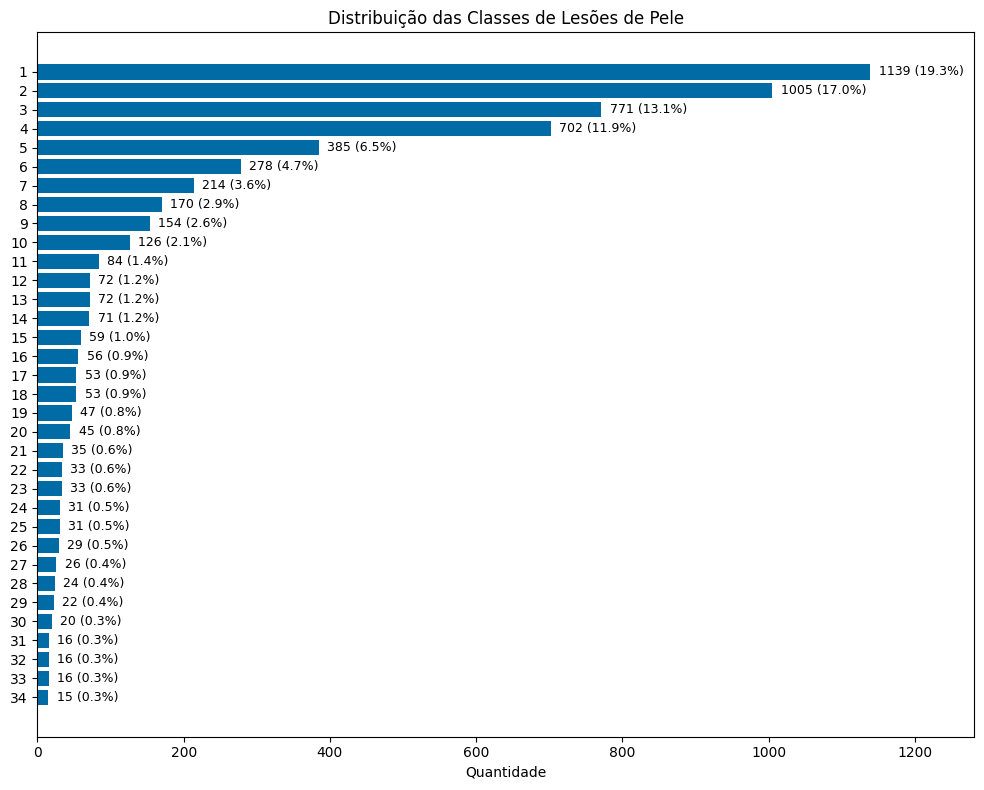
\includegraphics[width=1\columnwidth,keepaspectratio]{images/skin_lesion_classes.png}
    \label{fig:skin_lesion_classes}
    \fonte{Autoria própria.}
\end{figure}

\begin{table}[ht]
    \caption{\small Legenda das classes de lesões de pele.}
    \centering
    \begin{tabular}{l|l}
        \hline
        Número             & Classe de lesão de pele                                                  \\ \hline
        1                  & Lesões de pele que necessitam de avaliação presencial com dermatologista \\ \hline
        2                  & Câncer de pele Não Melanoma (CEC ou CBC)                                 \\ \hline
        3                  & Ceratose seborreica                                                      \\ \hline
        4                  & Ceratoses solares/actínicas                                              \\ \hline
        5                  & Nevo melanocítico                                                        \\ \hline
        6                  & Outras                                                                   \\ \hline
        7                  & Fotodano crônico                                                         \\ \hline
        8                  & Dermatite de Contato                                                     \\ \hline
        \multirow{2}{*}{9} & Lesões de pele que necessitam de avaliação presencial com dermatologista \\
                           & pediátrico                                                               \\ \hline
        10                 & Psoríase moderada a grave                                                \\ \hline
        11                 & Lesões de pele benignas com indicação de tratamento cirúrgico            \\ \hline
        12                 & Outras dermatoses                                                        \\ \hline
        13                 & Câncer de pele Melanoma                                                  \\ \hline
        14                 & Verrugas Virais                                                          \\ \hline
        15                 & Tineas                                                                   \\ \hline
        16                 & Psoríase leve                                                            \\ \hline
        17                 & Anexos/alopécias                                                         \\ \hline
        18                 & Pitiríase Versicolor                                                     \\ \hline
        19                 & Dermatite Atópica                                                        \\ \hline
        20                 & Acne                                                                     \\ \hline
        21                 & Asteatose Cutânea                                                        \\ \hline
        22                 & Melasma                                                                  \\ \hline
        23                 & Anexos/onicoses                                                          \\ \hline
        24                 & Escabiose                                                                \\ \hline
        25                 & Molusco Contagioso                                                       \\ \hline
        26                 & Foliculite                                                               \\ \hline
        27                 & Dermatite Seborreica                                                     \\ \hline
        28                 & Líquen simples crônico (Neurodermite)                                    \\ \hline
        29                 & Eczema de Estase                                                         \\ \hline
        30                 & Eczemas                                                                  \\ \hline
        31                 & Prurido                                                                  \\ \hline
        32                 & Rosácea                                                                  \\ \hline
        33                 & Colagenoses                                                              \\ \hline
        34                 & Estrófulo                                                                \\ \hline
    \end{tabular}
    \label{tab:skin_lesion_classes_legend}
    \fonte{Autoria própria}
\end{table}

\clearpage

\begin{figure}[ht]
    \centering
    \caption{\small Distribuição das classificações de risco em ordem decrescente.}
    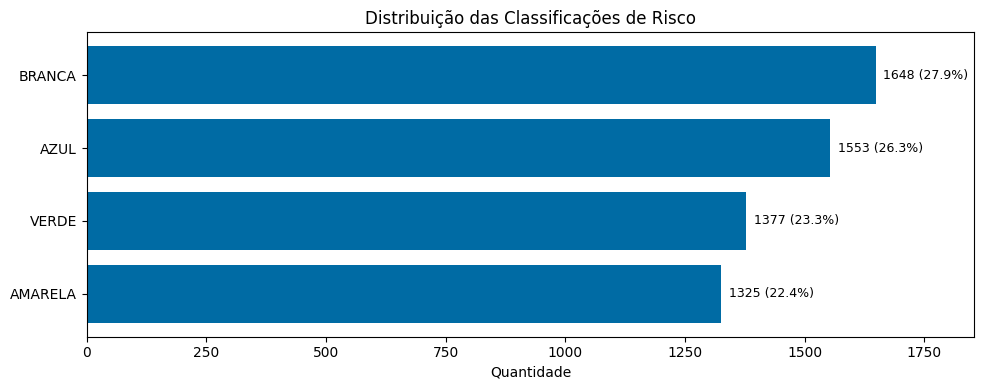
\includegraphics[width=0.9\columnwidth,keepaspectratio]{images/risk_classes.png}
    \label{fig:risk_classes}
    \fonte{Autoria própria.}
\end{figure}

\begin{table}[ht]
    \caption{\small Legenda das classificações de risco.}
    \centering
    \begin{tabular}{l|l}
        \hline
        Rótulo                   & Classificação de risco                              \\ \hline
        \multirow{2}{*}{BRANCA}  & BRANCA - SEM NECESSIDADE DE INTERVENÇÃO OU          \\
                                 & ACOMPANHAMENTO                                      \\ \hline
        AZUL                     & AZUL - TRATAMENTO NA UNIDADE BÁSICA DE SAÚDE (UBS)  \\ \hline
        VERDE                    & VERDE - AVALIAÇÃO CLÍNICO-CIRURGIA COM ESPECIALISTA \\ \hline
        \multirow{2}{*}{AMARELA} & AMARELA - ENCAMINHAMENTO COM PRIORIDADE PARA        \\
                                 & O AMBULATÓRIO DE REFERÊNCIA TERCIÁRIO               \\ \hline
    \end{tabular}
    \label{tab:risk_classes_legend}
    \fonte{Autoria própria}
\end{table}

Por fim, o conjunto de dados foi seccionado entre um conjunto de treinamento com 80\% dos dados e um de testes com
20\%. A divisão foi feita de forma estratificada com o método \textit{k-fold} com o agrupamento baseado nos \acp{ID}
dos exames. Este método de divisão garante que os pares de imagens e laudos de um mesmo exame fiquem no mesmo
subconjunto de dados, evitando o vazamento de dados, onde o modelo é treinado com pares extremamente similares aos
do conjunto de teste \cite{ghani2013proceedings}. No total, 4736 pares foram destinados ao conjunto de dados de
treinamento, enquanto 1167 pares foram para o conjunto de testes.

A criação de um terceiro conjunto de validação, como o utilizado na etapa inicial de desenvolvimento, foi considerada
desnecessária. A etapa final realiza apenas uma iteração de treinamentos com hiperparâmetros pré-definidos, evitando
a necessidade de validações e ajustes durante a execução desta etapa.

\clearpage

\begin{figure}[ht]
    \centering
    \caption{\small processo de sanitização e preparação do conjunto de dados. 1: Seleção das lesões de aproximação. 2:
    Sanitização e estruturação dos laudos. 3: Pareamento entre imagens e laudos. 4: Filtragem e remoção de campos
    desnecessários dos laudos. 5: Seccionamento do conjunto de dados.}
    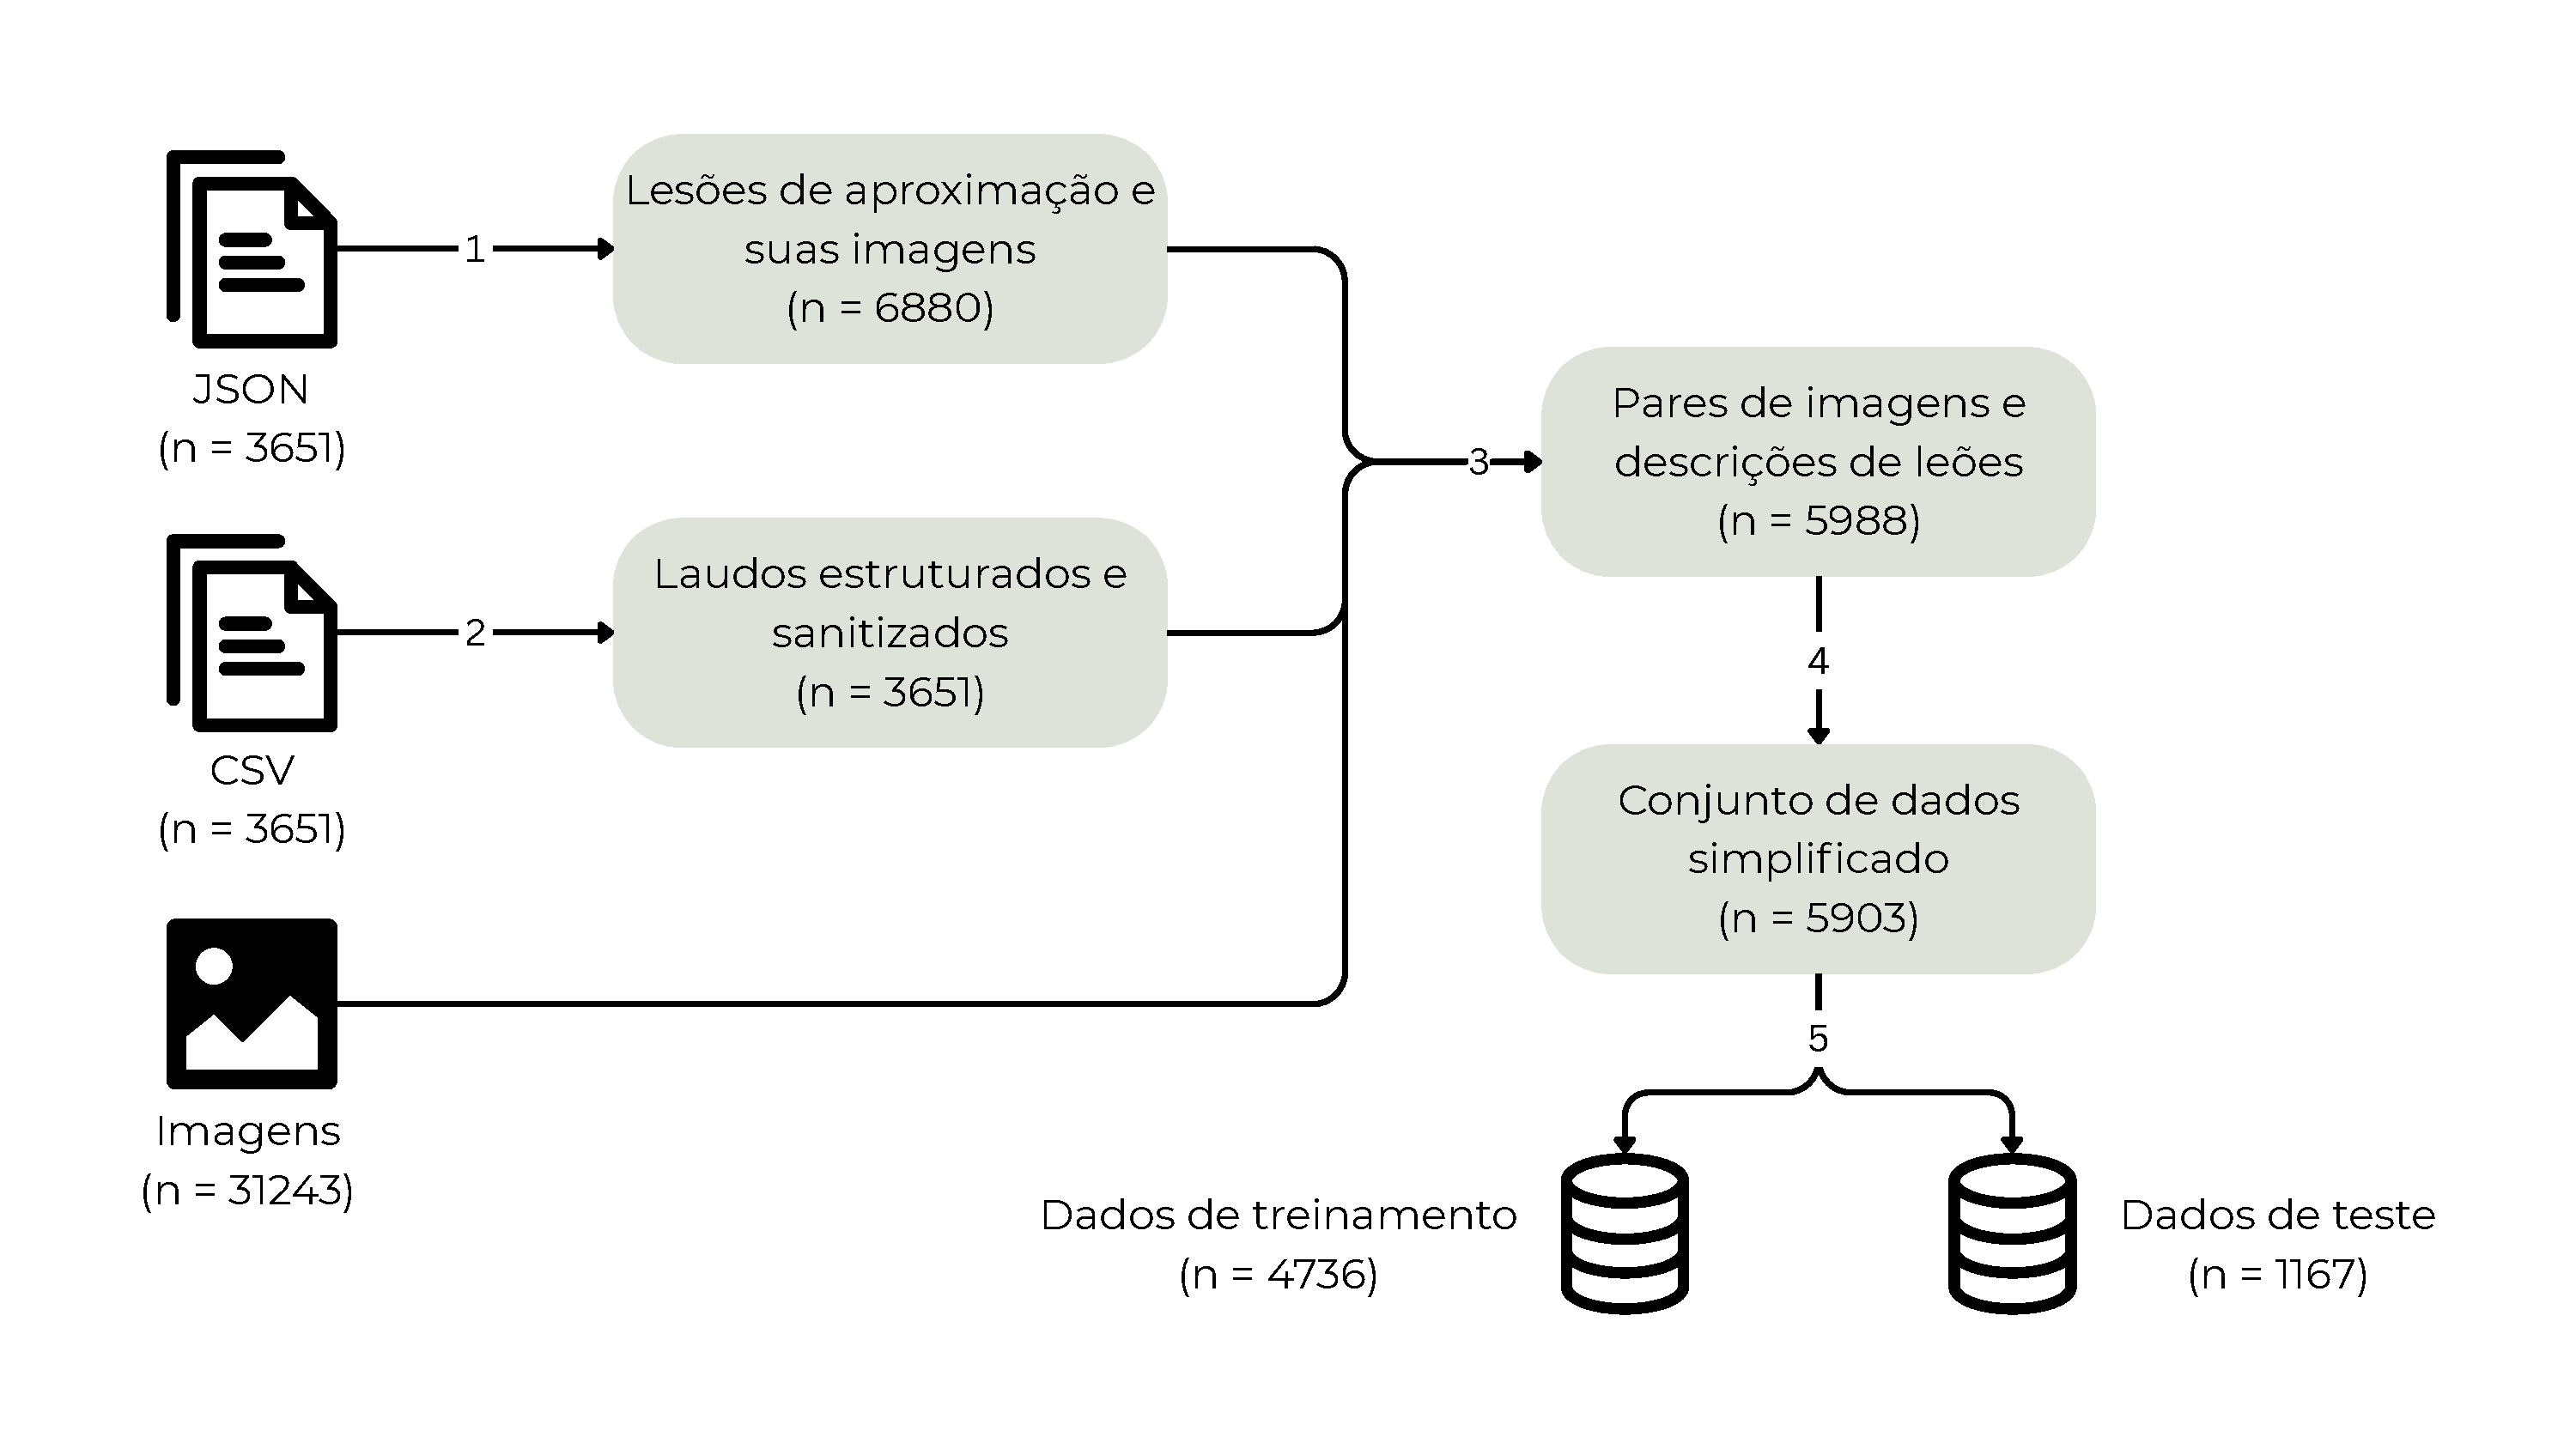
\includegraphics[width=1\columnwidth,keepaspectratio]{images/dataset_building.pdf}
    \label{fig:dataset_building}
    \fonte{Autoria própria.}
\end{figure}

\subsubsection{Construção do Conjunto de Dados no Modelo Conversacional}

Para a etapa final do desenvolvimento, o diálogo foi implementado em português. O padrão de pergunta e resposta pode
ser conferido abaixo:

\begin{dialogue}
    \speak{Usuário} Classifique a lesão de pele na imagem, informando a classificação da lesão e classificação de
    risco. \\
    Por fim, inclua uma breve conclusão sobre o diagnóstico. \\
    As opções de classificação de lesões de pele são: \textbf{<opções de lesões de pele>}. \\
    As opções de classificação de risco são: \textbf{<opções de classificações de risco>}. \\
    Utilize a seguinte formatação para a resposta: \\ \\
    Classificação: <...>. \\
    Classificação de risco: <...>. \\
    Conclusão sobre a lesão: <...>. \\
    Conclusão: <...>. \\
    \textbf{<imagem>} \\
    \speak{Modelo} Classificação: \textbf{<lesão de pele>}. \\
    Classificação de risco: \textbf{<classificação de risco>}. \\
    Conclusão sobre a lesão: \textbf{<conclusão sobre a lesão>}. \\
    Conclusão: \textbf{<conclusão>}.
\end{dialogue}

As opções de classificação de lesões de pele e de risco são oferecidas na pergunta, sendo que elas correspondem às
lesões e classificações de risco existentes no conjunto de dados. Para realizar o treinamento com \textit{fine-tuning},
o padrão de diálogo é preenchido com os dados do conjunto de treinamento.

\subsection{\textit{Fine-tuning}}

\subsection{Análise dos Resultados Finais}
